\documentclass{article}
% --- watermark (auto-inserted) ---
\usepackage{xcolor}
\usepackage{xfp}% \fpeval; in the kernel since 2022, harmless on older LaTeX
\usepackage{draftwatermark}
\newlength{\watermarkTextWidth}
\AddToHook{begindocument/end}{%
  \SetWatermarkText{\normalfont Generated by The Agentic Scientist}%
  \SetWatermarkFontSize{10pt}%
  \SetWatermarkLightness{0.85}%
  \settowidth{\watermarkTextWidth}{\normalfont\fontsize{10pt}{12pt}\selectfont Generated by The Agentic Scientist}%
  \edef\watermarkScale{\fpeval{0.8 * sqrt(\paperwidth**2 + \paperheight**2) / \watermarkTextWidth}}%
  \edef\watermarkAngle{\fpeval{atand(\paperheight/\paperwidth)}}%
  \SetWatermarkScale{\watermarkScale}%
  \SetWatermarkAngle{\watermarkAngle}%
}
% --- end watermark ---
 % For LaTeX2e
\usepackage{paper,times}

\usepackage{hyperref}
\usepackage{url}
\usepackage{graphicx}
\usepackage{booktabs}
\usepackage{amsmath,amssymb}
\usepackage{subcaption}

\title{Does Grokking Delay Depend on Width? An Inconclusive, Censoring-Aware Slope Test on Modular Addition}
\author{Anonymous authors}

\begin{document}
\maketitle

\begin{abstract}
Delayed generalization (``grokking'') on modular arithmetic has been explained through weight norm, circuit efficiency, and a lazy-to-rich transition in training dynamics; here we ask how the delay depends on model width, a quantity that these accounts relate to scale-dependent knobs.
We test one falsifiable prediction in a one-layer transformer trained with AdamW (weight decay $1.0$, full batch) on modular addition modulo $97$: that the delay between fitting the training pairs and generalizing to held-out pairs shrinks as width grows.
Delay is right-censored at $10{,}000$ steps, and a three-way interval rule (applied by us to the evaluator's reported interval) reads the 95\% seed-cluster bootstrap interval of the slope of $\ln(\text{delay})$ against $\log_2(\text{width})$ over widths $16$--$256$ with four seeds.
The measured slope is $-0.020$ with interval $[-0.585,\,0.354]$, so the verdict is \emph{inconclusive}; $40\%$ of the $20$ runs were censored, and the interval covers about two-fifths of the slopes that the delay floor and cap permit.
A single-seed reference trainer gives $-0.368$, inside the interval.
The evaluation itself was valid, so the result is a valid but inconclusive measurement rather than a failed run; the interval comes from only four seed clusters and its coverage is not guaranteed. We state what the result cannot say and which measurements would resolve it.
\end{abstract}

\section{Introduction}
\label{sec:intro}
In small algorithmic tasks such as modular addition, networks often fit the training split almost immediately and generalize to held-out pairs only after much longer training \citep{Power2022GrokkingGB}. Several accounts of this delay have been proposed: a mechanistic account in which a generalizing circuit forms gradually under weight decay \citep{Nanda2023ProgressMF}, a loss-landscape and weight-norm account \citep{Liu2022OmnigrokGB}, a circuit-efficiency account \citep{Varma2023ExplainingGT}, and a lazy-to-rich account of training dynamics \citep{Kumar2023GrokkingAT}. How the delay depends on \emph{model size} is a more practical question: it constrains these accounts and informs which model sizes are worth using in experiments on the phenomenon. A capacity-based reading predicts that wider models memorize sooner, and, if generalization time is less sensitive to width, that the delay changes systematically with width.

This paper reports a single, carefully scoped measurement of that kind. The setting is a one-layer transformer trained on modular addition modulo $p=97$ with a fixed training fraction, optimizer, and step limit, and the width $d$ is varied over $\{16,32,64,128,256\}$. The prediction under test is that the delay decreases with width, operationalized as the slope of $\ln(\text{delay})$ against $\log_2 d$ being negative with a 95\% seed-cluster bootstrap interval entirely below zero. We apply a three-way rule to the interval the evaluator reports: the prediction is read as \emph{supported} if the interval lies entirely below zero, \emph{refuted} if it lies at or above zero, and \emph{inconclusive} if it straddles zero (Figure~\ref{fig:overview}). The rule is our own operationalization; the evaluator reports only the slope and its interval.

The outcome is inconclusive. The sealed evaluation, run on four seeds at each of five widths, gives a slope of $-0.020$ with 95\% interval $[-0.585, 0.354]$. The evaluation was valid in the sense that it completed and passed the evaluator's validity checks (the evaluator labels it \texttt{qualified}); this status concerns the integrity of the measurement and does not mean that the width prediction was supported. Because a flat answer is easy to misread, much of this paper is about \emph{why} the measurement is inconclusive and how large an effect it could have resolved.

\paragraph{Contributions.} (i) We state precisely the delay statistic, its floor and censoring cap, the seed-cluster slope test, and the three-way interval rule we apply to the evaluator's reported interval (Section~\ref{sec:method}). (ii) We report the measured outcome with its uncertainty and its cross-check against a single-seed reference trainer (Section~\ref{sec:results}). (iii) We derive, from the protocol constants and the reported interval, the resolution limits of this design: the range of slopes the floor and cap allow, the fraction of that range covered by the interval, and the coarseness of a four-cluster bootstrap (Section~\ref{sec:resolution}). (iv) We list what the retained artifacts cannot support, including per-width delays, a mechanistic decomposition, and any isolation of the evaluated model's width-dependent parametrization (Section~\ref{sec:discussion}). We make no claim that delay is, or is not, width-dependent in modular addition.

\begin{figure}[t]
\centering
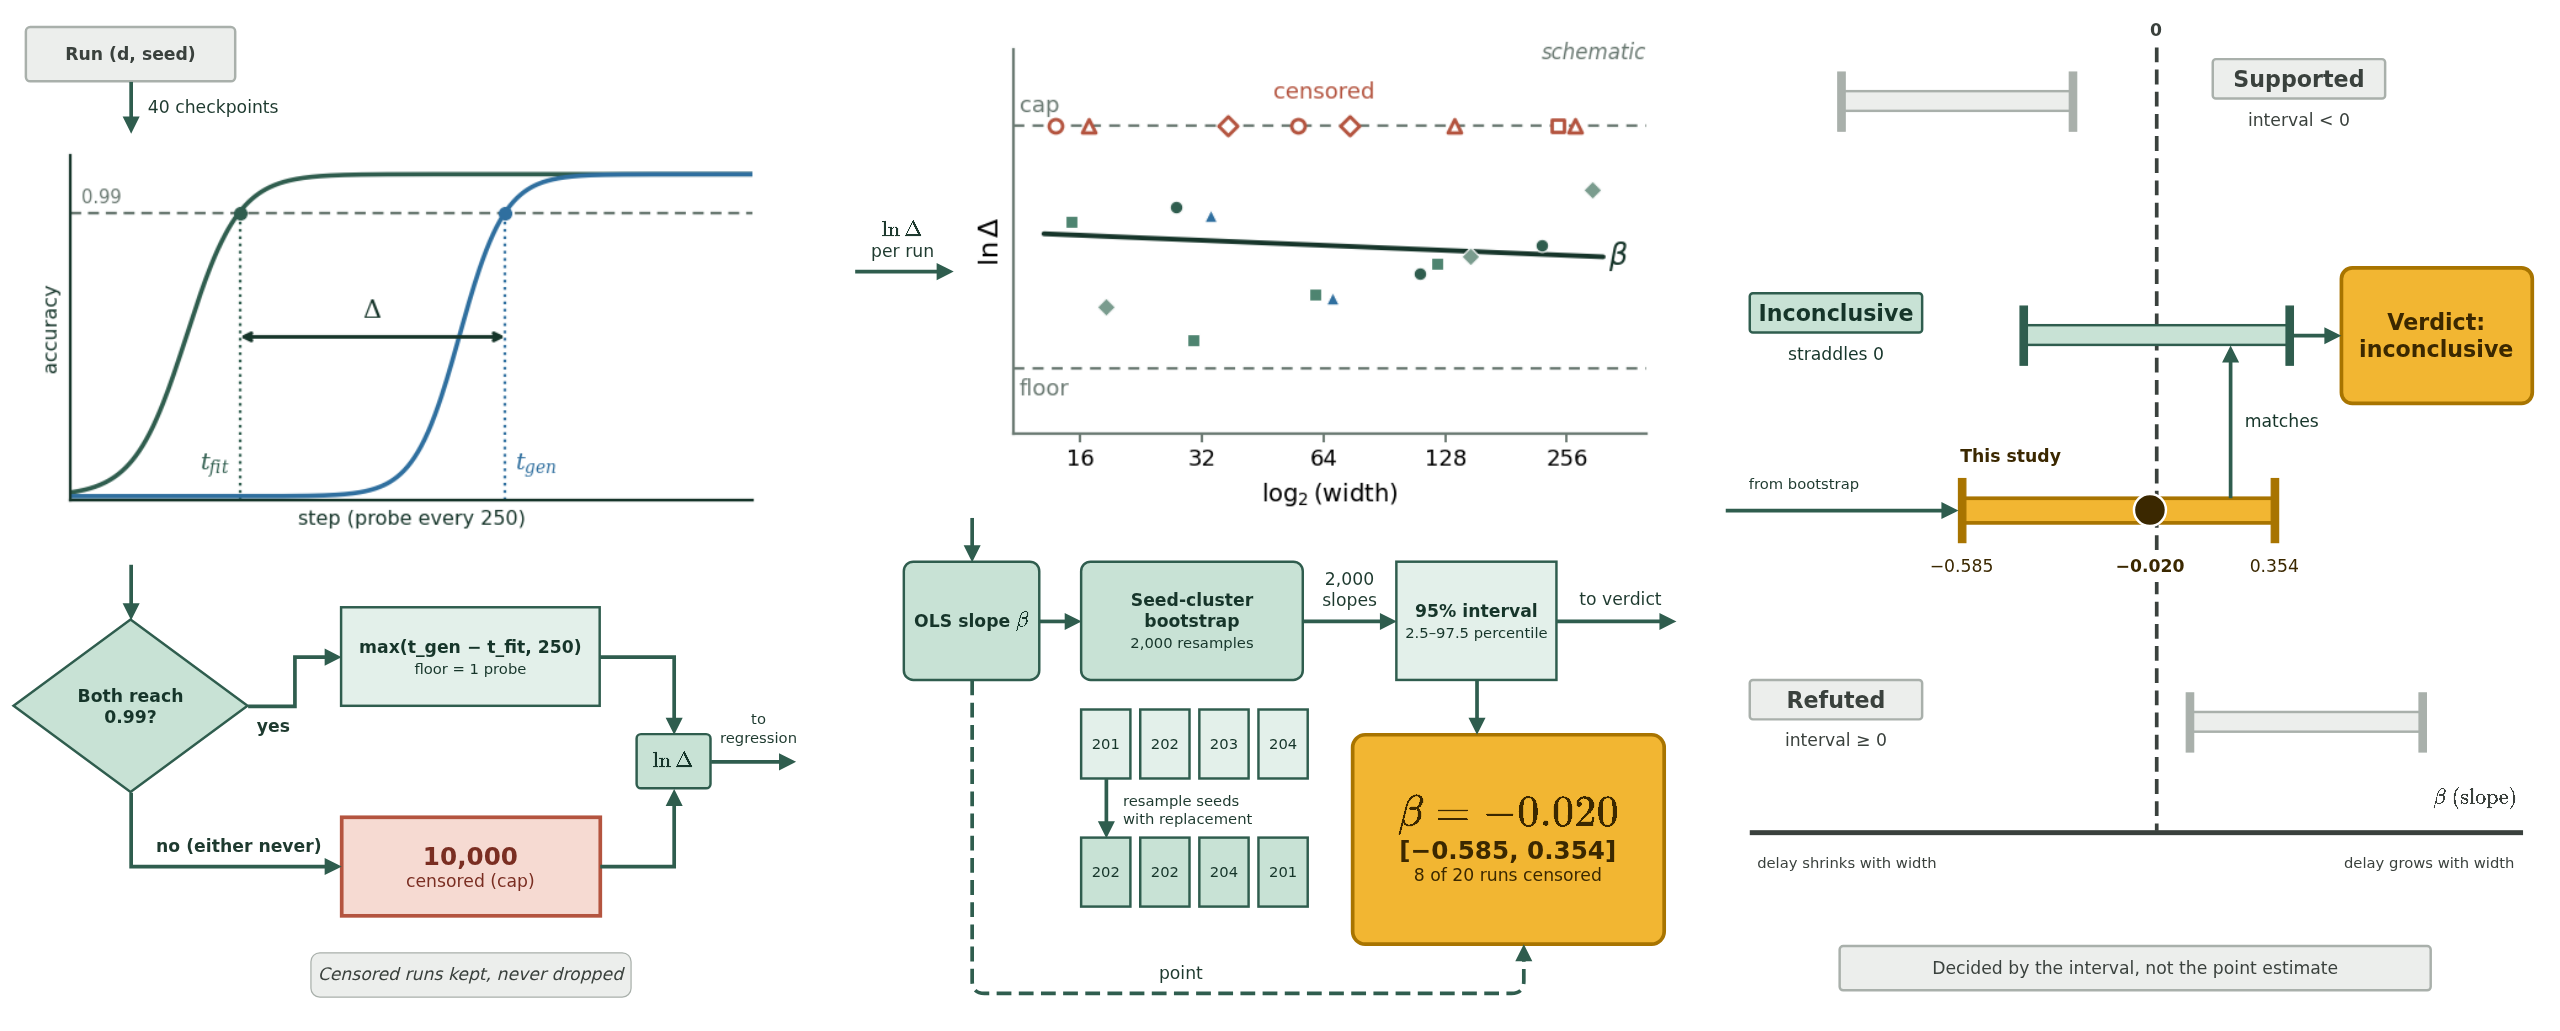
\includegraphics[width=\textwidth]{figures/protocol_overview.png}
\caption{Overview of the width-dependence test. Delay is the gap between the first checkpoint at which training accuracy reaches $0.99$ and the first at which held-out accuracy does, floored at one probe interval and set to the step limit if either threshold is never reached. The slope of $\ln$(delay) against $\log_2$(width) is estimated over five widths and four seeds, with a seed-cluster bootstrap interval; the interval, not the point estimate, determines the verdict. In this study the interval straddles zero and the verdict is inconclusive.}
\label{fig:overview}
\end{figure}

\section{Related Work}
\label{sec:related}
\paragraph{Grokking and its explanations.} \citet{Power2022GrokkingGB} report that small transformers trained on algorithmically generated tables, including modular arithmetic, reach high held-out accuracy long after fitting the training split. \citet{Nanda2023ProgressMF} analyze small transformers trained on modular addition mechanistically and define progress measures that track the formation of the generalizing circuit during training. \citet{Liu2022OmnigrokGB} analyze loss landscapes and weight norm and extend the phenomenon beyond algorithmic data; \citet{Varma2023ExplainingGT} explain grokking through circuit efficiency and test predictions of that account in training experiments; \citet{Kumar2023GrokkingAT} relate it to a transition from lazy to rich training dynamics, analyzed in a two-layer regression setting; \citet{Huang2024UnifiedVO} discuss grokking, double descent, and emergent abilities through the competition of circuits; and \citet{Davies2023UnifyingGA} place grokking and double descent in one framework. These accounts differ in which quantity should control the delay, and several involve scale-related knobs. Empirical studies have varied some of those knobs on modular arithmetic or related algorithmic tasks: \citet{Doshi2023ToGO} study modular arithmetic with corrupted labels and examine how generalization and memorization coexist under regularization; \citet{Thilak2022TheSM} associate grokking under adaptive optimizers with cyclic behavior of the last-layer norm; and \citet{Prieto2025GrokkingAT} attribute the absence of grokking without regularization to numerical instability in the softmax. We do not re-derive these findings, and none of them has, as far as their stated scope and our non-exhaustive reading indicate, measured delay against width under a fixed protocol, which is the quantity examined here; the present study does not test the accounts against each other.

\paragraph{Model size, memorization, and double descent.} Test error can vary non-monotonically with model size and training time \citep{Nakkiran2019DeepDD}; networks can fit random labels, so fitting the training set does not by itself imply generalization \citep{Zhang2016UnderstandingDL}; memorization of training data has been studied empirically during language-model training \citep{Tirumala2022MemorizationWO}, and a method for estimating how much information a model stores about data points has been proposed and measured on language models \citep{Morris2025HowMD}. These works motivate a capacity-based reading of the grokking delay, in which fitting time and generalization time depend differently on width. We use them only as motivation: the artifacts of this study do not record fitting time and generalization time separately.

\paragraph{Parametrization and optimizer scale.} The evaluated model contains width-dependent multipliers on hidden and output layers (Section~\ref{sec:model}), motivated by the observation that the step size a layer effectively receives under an adaptive optimizer depends on its parametrization. The width-aware parametrization literature makes this precise: \citet{Yang2021TensorPI} characterize a maximal-update parametrization in which hidden-layer features keep learning as width grows, and \citet{Yang2022TensorPV} show that hyperparameters such as the learning rate then transfer across widths. Our multipliers resemble this construction in spirit, but we do not claim that they implement it, and we did not check hyperparameter transfer; the point for this study is only that a width-dependent multiplier can change how fast wider models move, and so can mask or create a width slope. The role of effective learning rates under normalization has been studied in reinforcement learning \citep{Lyle2024NormalizationAE}, practical measures of dynamical richness have been proposed \citep{Nam2024DecouplingDR}, and decoupled weight decay, which we use, is introduced by \citet{Loshchilov2017DecoupledWD}. We do not measure the effect of these multipliers in isolation.

\paragraph{Relation to this work.} Rather than propose a new explanation, we examine what a censoring-aware slope test on one architecture and one task can and cannot resolve, and we report an inconclusive result in full.

\section{Method}
\label{sec:method}

\subsection{Problem setup and hypothesis}
\label{sec:setup}
\paragraph{Task.} Inputs are all $p^2=9{,}409$ ordered pairs $(a,b)$ with $a,b\in\{0,\dots,96\}$ and label $(a+b)\bmod 97$. For each seed, a random $40\%$ of pairs ($3{,}763$) forms the training split and the remaining $5{,}646$ pairs are held out; the evaluator, not the model, owns the split, the checkpoint schedule, and all metrics.

\paragraph{Delay.} Training runs for at most $T=10{,}000$ full-batch steps and is probed every $250$ steps, giving $40$ checkpoints at which accuracy is computed by the evaluator on all pairs. Let $t_{\mathrm{fit}}$ be the first checkpoint at which training accuracy is at least $0.99$, and $t_{\mathrm{gen}}$ the first at which held-out accuracy is at least $0.99$. The delay is
\begin{equation}
\Delta = \begin{cases} \max(t_{\mathrm{gen}}-t_{\mathrm{fit}},\,250) & \text{if both thresholds are reached,}\\ 10{,}000 & \text{otherwise (censored).}\end{cases}
\end{equation}
A run is censored if \emph{either} threshold is never reached. Censored runs keep the cap value and are never dropped or reweighted. The floor of one probe interval ($250$ steps) also applies when held-out accuracy crosses $0.99$ no later than training accuracy does. Both the floor and the cap therefore bound $\ln\Delta$ to $[\ln 250,\ln 10{,}000]$, a ratio of $40$.

\paragraph{Test statistic and decision rule.} With widths $d\in\{16,32,64,128,256\}$ and seeds $s\in\{201,202,203,204\}$ the statistic is the ordinary-least-squares slope $\beta$ of $\ln\Delta_{d,s}$ on $\log_2 d$ over the $20$ pairs. Its interval is the 2.5--97.5 percentile range of $2{,}000$ bootstrap slopes in which seeds are resampled with replacement and each resampled seed contributes all five of its widths (a cluster bootstrap over seeds, with a fixed resampling seed; \citealp{Cameron2015APG}). The verdict is obtained by applying a three-way rule to the evaluator's reported interval; the rule is our own operationalization of the prediction (implemented in \texttt{scripts/derive\_resolution.py}); the evaluator emits only the interval and the other metrics, and we make no claim about when the rule was fixed. The prediction ``delay decreases with width'' is \emph{supported} if the interval lies entirely below zero, \emph{refuted} if it lies at or above zero, and \emph{inconclusive} if it straddles zero or the evidence is incomplete. The claim is restricted to the tested setting (modular addition, one training fraction, AdamW with weight decay $1.0$, full batch, one layer, the five widths) and makes no statement about other operations, moduli, optimizers, depths, or larger models.

\paragraph{Caveat on few clusters.} The cluster-robust inference literature documents that inference with a small number of clusters can be unreliable, and that refinements to the basic cluster bootstrap, such as the wild cluster bootstrap-$t$, can improve coverage \citep{Cameron2008BootstrapBasedIF,Cameron2015APG}. We use the plain percentile interval with four clusters as the evaluator reports it, make no claim of nominal coverage, and treat the interval as a coarse summary of seed-to-seed variability rather than an exact confidence statement.

\paragraph{What the interval does and does not capture.} Each seed fixes both the train/held-out split and the weight initialization, and the design has exactly one run per seed and width. Resampling seeds therefore propagates split and initialization variability jointly, and a seed is the unit of replication; run-to-run nondeterminism within a seed is not separated from it, and cannot be, since no seed is repeated at a width in the sealed design. Because the design is balanced, the pooled OLS slope equals the slope fitted to the width-wise means of $\ln\Delta$, and the bootstrap interval is the percentile range of that quantity over seed resamples.

\subsection{Evaluated model}
\label{sec:model}
The evaluated configuration is a one-layer, four-head transformer with width $d$ (the model dimension), an MLP of hidden size $4d$ with ReLU, no normalization layers, a learned embedding for the $97$ residues plus a separator token ``$=$'' appended as the third input position, and a learned positional embedding. Attention is non-causal and only the representation at the final position is read out; the implementation computes queries, residual stream, and MLP for that position only, which by inspection of the one-layer architecture gives the same outputs as processing all positions. Writing $z_i=E[x_i]+P_i$ for the embedded tokens $x_1,x_2,x_3{=}$``$=$'', the evaluated model computes
\begin{equation}
h=z_3+W_O\,\mathrm{Attn}(z_1,z_2,z_3),\qquad h'=h+W_2\,\mathrm{ReLU}(W_1h+b_1)+b_2,\qquad \text{logits}=m_d\,W_U\,h',
\end{equation}
with $W_\ast=m_dV_\ast$ for the attention and MLP matrices (Modification 3 below; $m_d=1$ recovers the plain parametrization) and $W_U$ the unembedding. The parameter count is $12d^2+(2p+9)d$, from $6{,}320$ at $d=16$ to $838{,}400$ at $d=256$, within the $10^6$ budget (Appendix~\ref{sec:si-model}).

Relative to the evaluator's stock model, the configuration has three modifications, all visible in the source (\texttt{source\_evidence/frozen\_model/program.py}):
\begin{enumerate}
\item \emph{Smaller initial weights.} All hidden and output weight matrices are multiplied by $0.5$ at initialization.
\item \emph{Width-aware output scaling.} The unembedding weights are additionally halved at initialization, and the logits are multiplied by $m_d=(128/d)^{1/2}$.
\item \emph{Hidden-layer reparametrization.} Each hidden matrix is written $W=m_d V$ with the same multiplier $m_d$, and $V$ is initialized as $W_{\mathrm{init}}/m_d$ so that the function at initialization is unchanged. The optimizer updates $V$, and decoupled weight decay acts on $V$. The code comments state the intent: under Adam-type updates $V$ moves at about the learning rate per step, so $W$ moves at about $m_d$ times the learning rate, which is meant to compensate for width in the effective step size.
\end{enumerate}
The multiplier is $2.83, 2.0, 1.41, 1.0, 0.71$ at $d=16,\dots,256$. The exponents ($0.5$) and the reference width ($128$) are fixed constants in the model source, not adjusted during the final evaluation. The training workload is dictated by the evaluator: AdamW with learning rate $10^{-3}$, $\beta=(0.9,0.98)$, decoupled weight decay $1.0$, full-batch updates on all $3{,}763$ training pairs, and $10{,}000$ steps. We refer to this configuration as the \emph{evaluated model}.

\subsection{Reference trainer, controls, and validity}
\label{sec:controls}
\paragraph{Reference trainer.} The evaluator also trains its own stock transformer with the same optimizer settings and no modifications (no initialization shrinkage, no multipliers, all positions processed), using the first final seed ($201$) at each of the five widths. The OLS slope of $\ln\Delta$ on $\log_2 d$ over these five single-seed delays is the reference slope. It has no interval.

\paragraph{Controls.} Two control runs at width $64$ and seed $201$ check that the measurement does not manufacture generalization: one trains on training labels that have been permuted (at least $90\%$ of labels changed) and one performs zero optimizer steps. A control fails if its held-out accuracy ever exceeds $0.10$; chance level for $97$ classes is about $0.010$.

\paragraph{Validity.} The evaluator marks the final evaluation valid (\texttt{qualified}, status \texttt{completed}) when, according to its source, all episodes completed, the compute and call budgets were respected, the controls passed, and at least one run fit the training data to $0.99$. Only these three status fields are retained in the artifacts; per-condition diagnostics beyond them are not, so we treat any finer breakdown as unknown. Diagnostics reported by the evaluated model itself are untrusted and not used: every accuracy, delay, control, and statistic below is computed by the evaluator from returned predictions.

\subsection{Scope of the retained evidence}
\label{sec:scope}
The retained final artifacts consist of the aggregate metrics listed in Section~\ref{sec:results} and one record per seed (mean validation-accuracy score and wall-clock time). \emph{Per-width and per-seed delays, fitting and generalization steps, and per-width censoring flags are not retained}, so we cannot show a delay-versus-width plot, and we do not infer one. Separately, a development evaluation on a different data plane (modulus $53$, training fraction $0.5$, widths $32,64,128$, $6{,}000$ steps, two seeds) was used when configuring the evaluated model; its results are reported only as descriptive context in Appendix~\ref{sec:si-dev} and never mixed with the sealed result.

\section{Results}
\label{sec:results}

\subsection{Main result: the slope test is inconclusive}
The sealed evaluation completed with status \texttt{qualified}. Its aggregate metrics are listed in Table~\ref{tab:metrics}.
% @evidence[[paper_data.json#final_evaluation.metrics]]
The slope of $\ln\Delta$ on $\log_2 d$ is $-0.020$, with 95\% seed-cluster bootstrap interval $[-0.585,\,0.354]$. Because the interval contains zero, the interval rule returns \emph{inconclusive}: the prediction that delay decreases with width is neither supported nor refuted. A point estimate of $-0.020$ corresponds to a fitted multiplicative change of $0.980$ in delay per doubling of width, and the interval to factors between $0.557$ and $1.425$; over the full $16\to256$ range the fitted factors are $0.924$ with interval $[0.096, 4.12]$.
% @evidence[[derived/resolution.json#per_doubling_factor]] @evidence[[derived/resolution.json#range_factor_256_vs_16]]
That is, the data are compatible with a delay roughly $10$ times shorter at width $256$ than at $16$, with no change, and with a delay about $4$ times longer.

\begin{table}[t]
\centering
\caption{Sealed final evaluation: aggregate metrics (four seeds $\times$ five widths $=20$ runs, plus two controls). ``Score'' is the mean over seeds and widths of the area under the held-out-accuracy curve over the $40$ checkpoints; it does not use the $0.99$ threshold.}
\label{tab:metrics}
\small
\begin{tabular}{lr}
\toprule
Quantity & Value \\
\midrule
Slope of $\ln\Delta$ on $\log_2 d$ (point) & $-0.020$ \\
95\% seed-cluster bootstrap interval & $[-0.585,\,0.354]$ \\
Verdict under interval rule & inconclusive \\
Reference-trainer slope (seed 201 only, no interval) & $-0.368$ \\
Censored fraction of the 20 runs & $0.40$ ($8$ runs) \\
Control maximum held-out accuracy (ceiling $0.10$) & $0.012$ \\
Missing episodes & $0$ \\
Score (mean held-out-accuracy AUC) & $0.729$ \\
\bottomrule
\end{tabular}
\end{table}
% @evidence[[paper_data.json#final_evaluation.metrics]]

\begin{figure}[t]
\centering
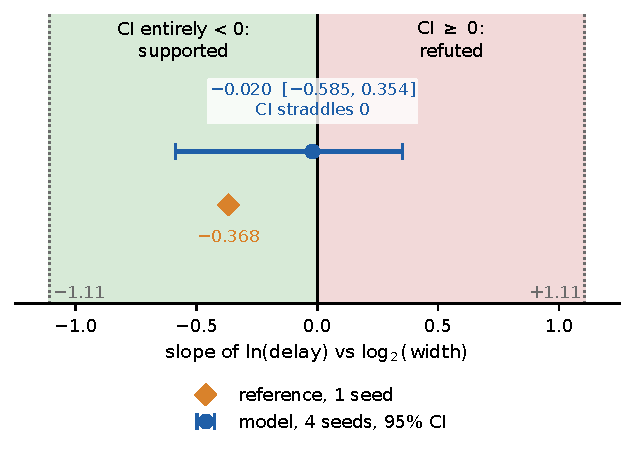
\includegraphics[width=0.8\textwidth]{figures/slope_interval_vs_decision_rule.pdf}
\caption{The estimated slope and its 95\% interval against the three decision regions. The interval straddles zero, so the verdict is inconclusive. The single-seed reference slope lies inside the interval. Dotted lines mark the largest slope magnitude attainable ($1.107$) when every width-wise mean delay is confined to $[250, 10{,}000]$.}
\label{fig:slope}
\end{figure}

\subsection{Resolution of the design}
\label{sec:resolution}
An inconclusive verdict is informative only relative to the effects the design could have resolved. Three properties of the protocol, all computed from its constants and the reported interval (Table~\ref{tab:resolution}), limit that resolution.
% @evidence[[derived/resolution.json]] @evidence[[source_evidence/workload/final_manifest.json#full]]

\emph{Bounded dynamic range.} In this balanced design the slope is a fixed linear contrast of the width-wise mean log-delays $m_d=\tfrac14\sum_s\ln\Delta_{d,s}$:
\begin{equation}
\beta=\sum_{d} w_d\,m_d,\qquad (w_{16},\dots,w_{256})=(-0.2,\,-0.1,\,0,\,0.1,\,0.2),
\end{equation}
that is, $\beta=0.2\,(m_{256}-m_{16})+0.1\,(m_{128}-m_{32})$; the middle width carries no weight, and the verdict depends only on how the two widest models compare with the two narrowest. Because every $m_d\in[\ln 250,\ln 10{,}000]$, $|\beta|\le 0.3\ln 40=1.107$, attained by a step profile; a delay falling log-linearly from the cap at $d=16$ to the floor at $d=256$ would give $-0.922$. The interval has width $0.939$ and covers $42\%$ of the attainable range $[-1.107,1.107]$. Its lower arm extends $0.565$ below the point estimate and its upper arm $0.374$ above.

\emph{Distance to a supported verdict.} Keeping the upper arm of the interval unchanged, a verdict of supported would have required a point estimate below $-0.374$. The reference slope ($-0.368$) is slightly above that value; with the same upper arm it would give an upper endpoint of $+0.006$, still straddling zero. This is arithmetic on the observed spread, not a forecast: the spread of a different point estimate would differ.

\emph{A coarse bootstrap.} With four seeds there are only $\binom{7}{4}=35$ distinct multisets of seeds to resample, and a fraction $4/4^4=1/64$ of draws consist of a single seed repeated four times. The $2{,}000$ resamples therefore estimate a discrete distribution with at most $35$ support points; the percentile endpoints $-0.585$ and $0.354$ should be read as coarse, and the coverage of an interval built from four clusters is not guaranteed to be nominal.

\begin{table}[t]
\centering
\caption{Quantities derived from the protocol constants and the reported interval (not additional measurements).}
\label{tab:resolution}
\small
\begin{tabular}{lr}
\toprule
Quantity & Value \\
\midrule
Delay floor / cap (steps) & $250$ / $10{,}000$ \\
Largest attainable $|\text{slope}|$ (step profile) & $1.107$ \\
Slope of a log-linear cap-to-floor profile & $-0.922$ \\
Interval width & $0.939$ \\
Interval width as fraction of $[-1.107, 1.107]$ & $0.42$ \\
Interval arms below / above the point estimate & $0.565$ / $0.374$ \\
Per-doubling delay factor: point [interval] & $0.980$ [$0.557$, $1.425$] \\
$16\to256$ delay factor: point [interval] & $0.924$ [$0.096$, $4.12$] \\
$16\to256$ delay factor at the reference slope & $0.230$ \\
Distinct bootstrap seed multisets & $35$ \\
\bottomrule
\end{tabular}
\end{table}

\subsection{Censoring}
Forty percent of the $20$ runs ($8$ runs) were censored at the step limit and entered the regression with the cap value $10{,}000$. Censoring has two consequences. First, because censored delays are replaced by the largest permitted value, any real dependence whose long-delay end is censored is compressed, so the fitted slope is biased toward zero when long delays concentrate at one end of the width range. Second, \emph{censored} here covers two different events, held-out accuracy never reaching $0.99$ and training accuracy never reaching $0.99$; the retained artifacts do not say which occurred or at which widths, so they cannot separate delayed generalization from failure to fit. The score in Table~\ref{tab:metrics} offers a threshold-free view: averaged over widths and seeds, held-out accuracy integrated over the $40$ checkpoints is $0.729$, so the runs on average generalize to a substantial degree within the window, but this aggregate does not locate where in the width range that happens.
% @evidence[[paper_data.json#final_evaluation.metrics.censored_fraction]] @evidence[[derived/resolution.json#n_censored_runs]]

\subsection{Seed-level variability}
The four seeds differ considerably in the score (Table~\ref{tab:seeds}), from $0.607$ to $0.860$ with mean $0.729$ and sample standard deviation $0.104$. We report this as variability across seeds, not as a performance comparison: each seed's score averages five widths, and a single seed supplies one run at every width. That the seed-to-seed spread is large relative to the quantities of interest is consistent with the wide interval for the slope, although the artifacts do not allow a variance decomposition across widths.
% @evidence[[paper_data.json#final_evaluation.evaluation_evidence.episodes]] @evidence[[derived/resolution.json#seed_score_sd]]

\begin{table}[t]
\centering
\caption{Seed-level records from the sealed evaluation. Score: mean over the five widths of the held-out-accuracy AUC. Wall-clock time is summed over all episodes with that seed; seed 201 also includes the two control runs.}
\label{tab:seeds}
\small
\begin{tabular}{lrr}
\toprule
Seed & Score & Wall-clock (s) \\
\midrule
201 & $0.607$ & $2{,}468$ \\
202 & $0.733$ & $1{,}894$ \\
203 & $0.717$ & $2{,}062$ \\
204 & $0.860$ & $1{,}943$ \\
\midrule
Mean $\pm$ s.d. & $0.729 \pm 0.104$ & \\
\bottomrule
\end{tabular}
\end{table}
% @evidence[[paper_data.json#final_evaluation.evaluation_evidence.episodes]]

\subsection{Cross-check against the reference trainer}
The reference trainer, run on seed $201$ only, gives a slope of $-0.368$, a fitted $16\to256$ delay factor of $0.230$, and lies inside the interval, $23\%$ of the way from its lower endpoint to its upper. The evaluated model's point estimate is $0.348$ larger (less negative). We draw no conclusion about this difference: the reference slope is one seed with no uncertainty, five points define it, and the evaluated model differs from the reference in three simultaneous ways (Section~\ref{sec:model}). The comparison also does not establish that the multipliers weaken the width dependence: that would require both variants to be run with several seeds under the same protocol, which was not done.
% @evidence[[paper_data.json#final_evaluation.metrics.reference_delay_log_slope]] @evidence[[derived/resolution.json#reference_position_in_ci_fraction_from_low]]

\subsection{Validity checks and development-plane context}
The two controls stayed far below their ceiling (maximum held-out accuracy $0.012$ against a ceiling of $0.10$), no episodes were missing, and the evaluator reports a completed, valid evaluation. These checks support the integrity of the measurement. They do not bear on the width question, and a valid measurement can be inconclusive.

For context, three configurations that differ cumulatively by the three modifications of Section~\ref{sec:model} were evaluated on the separate development plane with two seeds each, with scores $0.798$, $0.828$, and $0.850$ and $4$, $6$, and $4$ of $6$ runs censored (Appendix~\ref{sec:si-dev}). Differences between configuration means are no larger than the seed-to-seed spreads within a configuration, the plane differs from the sealed one in modulus, training fraction, widths, step limit, and seeds, and no slope interval was computed; we therefore draw no inference from them.
% @evidence[[derived/resolution.json#search]]

\section{Discussion and Limitations}
\label{sec:discussion}

\paragraph{Relation to the explanations of grokking.} Each account in Section~\ref{sec:related} associates the delay with a quantity that can depend on width or parametrization: initial weight norm and the loss landscape, the relative efficiency of memorizing and generalizing circuits, and the position on the lazy-to-rich axis. The evaluated model touches the last two knobs directly: its initial weights are shrunk by half, which the source comments describe as aimed at reducing lazy-regime memorization, and its multipliers change how large a step each layer takes at a given width. A clear width slope from this model could therefore reflect the multipliers rather than width alone, and a flat slope could reflect their compensating a stock-model dependence. This is why the isolating comparison with a matched stock model (Section~\ref{sec:discussion}, item iv) matters more than a further estimate of the slope for the evaluated model alone.

\paragraph{Alternative readings that the data cannot separate.} The interval is compatible with four readings (Table~\ref{tab:readings}). (a) \emph{Little or no width dependence} over $16$--$256$ in this setting. (b) \emph{A real negative dependence masked by censoring and noise}: cap-compressed delays and four seeds could produce a flat-looking slope. (c) \emph{Compensation by the width-aware multipliers}: if the hidden and output multipliers equalize effective step sizes across width, a dependence present in the stock model could be reduced in the evaluated one; the single-seed reference slope ($-0.368$) is more negative than the point estimate, but it is one seed without an interval and does not by itself support this reading. (d) \emph{Dependence that is non-monotone in $\ln d$}, which a linear slope cannot register. Each reading predicts something different about per-width delays and censoring flags, which are exactly the quantities not retained.

\begin{table}[t]
\centering
\caption{What each reading of the interval would imply for quantities that are not retained in the artifacts. None of these can be checked with the available records.}
\label{tab:readings}
\small
\begin{tabular}{p{0.22\textwidth}p{0.36\textwidth}p{0.30\textwidth}}
\toprule
Reading & Implication for per-width delays & Implication for censoring \\
\midrule
(a) Little or no width dependence & Similar delays across widths, within seed noise & Censored runs not concentrated at either end \\
(b) Negative dependence masked by cap and noise & Longer delays at narrow widths, partly hidden at the cap & Censored runs concentrated at narrow widths \\
(c) Compensation by multipliers & Matched stock-model runs show a steeper slope than evaluated-model runs on the same seeds & Differs between the two models at the same widths \\
(d) Non-monotone in $\ln d$ & Extremal delay at an intermediate width; contrast $\beta$ near zero & Censoring at both ends or in the middle \\
\bottomrule
\end{tabular}
\end{table}

\paragraph{Threshold and time-grid sensitivity.} The delay is read off a $250$-step grid with a $0.99$ threshold on both accuracies, so it is blind to differences below one probe interval and sensitive to where a run plateaus. The development evaluation shows how this can matter: all six runs of one configuration were censored even though their mean final held-out accuracy was $0.944$ (Appendix~\ref{sec:si-dev}), and the retained records do not show whether that censoring came from a missed training threshold or a missed held-out threshold, or how close individual runs came to $0.99$. We did not vary the threshold or the grid in the sealed evaluation, so we cannot say how the slope would change under, for example, a $0.95$ threshold, and the retained artifacts do not allow it to be recomputed.

\paragraph{What would resolve it.} Without claiming these were performed: (i) report per-width, per-seed delays with explicit censoring flags and the reason for censoring (not fitting vs.\ not generalizing); (ii) analyze delays as censored data instead of imputing the cap (survival-analysis regression, e.g.\ \citealp{Cox1972RegressionMA}, handles right-censored outcomes directly, although we did not apply it), or raise the step limit until few runs are censored; (iii) use more seeds, so that the bootstrap has more than $35$ distinct resamples; (iv) run the multipliers' exponent at $0$ and $0.5$ under the same protocol to isolate their effect (no result for such a sweep exists in the retained artifacts); (v) vary the training fraction, the modulus, and the weight decay, which determine the delay in the accounts reviewed in Section~\ref{sec:related}; and (vi) record fitting and generalization steps separately to test the capacity-based reading directly.

\begin{table}[t]
\centering
\caption{Claims and their status under this study's evidence.}
\label{tab:claims}
\small
\begin{tabular}{p{0.46\textwidth}p{0.17\textwidth}p{0.25\textwidth}}
\toprule
Claim & Status & Basis \\
\midrule
Delay decreases with width in this setting & Not established & Interval $[-0.585,0.354]$ contains $0$ \\
Delay is independent of width in this setting & Not established & Same interval also contains slopes down to $-0.585$ \\
The measurement was valid & Supported & Completed evaluation, controls $0.012$ vs.\ ceiling $0.10$, no missing episodes \\
A substantial share of runs is censored & Supported & $8$ of $20$ runs \\
The multipliers weaken or remove a width dependence & Not tested & Reference slope has one seed, no interval, no matched ablation \\
Fitting time and generalization time scale differently with width & Not testable & Not retained in the artifacts \\
Findings carry over to other moduli, fractions, operations & Not tested & One configuration only \\
\bottomrule
\end{tabular}
\end{table}

\paragraph{Limitations.} Table~\ref{tab:claims} summarizes which claims the evidence does and does not support. The evidence concerns one operation, one modulus ($97$), one training fraction ($0.4$), one optimizer setting, a single layer, and widths $16$--$256$ (up to $0.84\times 10^6$ parameters). The evaluated model contains three simultaneous modifications relative to the stock model, so even a clear slope would not be attributable to any one of them; sequential changes made during development support at most comparisons between whole configurations. The reference slope has one seed. The seed-cluster interval rests on four seeds. Censoring merges two events. The development-plane numbers come from a different workload with two seeds. We did not test the explanations in Section~\ref{sec:related}, did not run any weight-norm, circuit-level, or lazy-to-rich diagnostics, and did not run ablations of the three modifications. A valid evaluation does not imply scientific support for the prediction; the verdict is \emph{inconclusive}, and the design's limits above, rather than a demonstrated absence of effect, are the most defensible reading.

\section{Conclusion}
\label{sec:conclusion}
We tested whether the grokking delay of a one-layer transformer on modular addition decreases with width, using a censoring-aware slope test with a seed-cluster bootstrap interval. The sealed evaluation was valid and gave a slope of $-0.020$ with interval $[-0.585, 0.354]$ over widths $16$--$256$ and four seeds, so the prediction is neither supported nor refuted. Forty percent of runs were censored at the step limit, the interval covers about two-fifths of the slopes that the delay floor and cap allow, and a four-cluster bootstrap has only $35$ distinct resamples. A single-seed reference trainer gave $-0.368$, inside the interval. We therefore do not claim that delay depends on width, nor that it does not, and we do not attribute the difference between the reference and the evaluated model to any of its modifications. The practical lesson is a measurement one: for a delay statistic with a floor and a censoring cap, report per-width delays and censoring flags, use enough seeds that the cluster bootstrap has a rich resampling support, and treat the attainable slope range as part of the result. The per-width records, the isolating ablation of the multipliers, and sweeps over training fraction and weight decay would turn this inconclusive result into a testable one.

\clearpage
\bibliography{references}
\bibliographystyle{paper}

\clearpage
\appendix
\section{Supplementary Information}

\subsection{Protocol and hyperparameters}
\label{sec:si-protocol}
Table~\ref{tab:si-protocol} lists the workloads of the sealed evaluation and of the development evaluation, as specified in the evaluator's workload manifests (\texttt{source\_evidence/workload/}).
% @evidence[[source_evidence/workload/final_manifest.json]] @evidence[[source_evidence/workload/search_manifest.json]]

\begin{table}[h]
\centering
\caption{Workloads. The evaluator owns all items; the evaluated model receives only the training rows.}
\label{tab:si-protocol}
\small
\begin{tabular}{lll}
\toprule
 & Sealed final evaluation & Development evaluation \\
\midrule
Operation, modulus $p$ & addition, $97$ & addition, $53$ \\
Training fraction & $0.4$ ($3{,}763$ pairs) & $0.5$ \\
Widths $d$ & $16,32,64,128,256$ & $32,64,128$ \\
Seeds & $201$--$204$ & $101,102$ \\
Step limit / probe interval & $10{,}000$ / $250$ & $6{,}000$ / $300$ \\
Control width & $64$ & $64$ \\
Optimizer & \multicolumn{2}{c}{AdamW, lr $10^{-3}$, $\beta=(0.9,0.98)$, weight decay $1.0$, full batch} \\
Heads, layers & \multicolumn{2}{c}{$4$, $1$} \\
Fit / generalization threshold & \multicolumn{2}{c}{$0.99$ accuracy} \\
Bootstrap (final only) & $2{,}000$ seed-cluster resamples & -- \\
\bottomrule
\end{tabular}
\end{table}

The final evaluation made $1{,}804$ calls to the evaluated model (limit $2{,}200$; $22$ episodes, each a reset, a data load, and $40$ train/predict pairs) and took $11{,}764$\,s of wall-clock time including the reference trainer.
% @evidence[[derived/resolution.json#compute]] @evidence[[source_evidence/final/final_manifest.json#compute_usage]]

\subsection{Evaluated model: constants and parameter counts}
\label{sec:si-model}
Table~\ref{tab:si-model} gives the width-dependent constants and parameter counts of the evaluated model. The parameter count follows from the layer shapes in the source: embeddings $(p+1)d$, positional embedding $3d$, attention projections $3d^2+d^2$ (no bias), MLP $4d^2+4d$ and $4d^2+d$, unembedding $pd$ (no bias), totalling $12d^2+(2p+9)d$. The initial-weight scale ($0.5$), the unembedding scale ($0.5$), the reference width ($128$), and both exponents ($0.5$) are constants in the source. The code comments state that offline selection was not possible for the output-scaling, unembedding-scale and hidden-exponent defaults; the comments on the initial-weight scale and the reference width say nothing about how they were chosen.
% @evidence[[source_evidence/frozen_model/program.py]] @evidence[[derived/resolution.json#params_by_width]] @evidence[[derived/resolution.json#hidden_and_output_multipliers]]

\begin{table}[h]
\centering
\caption{Parameter count and multiplier $m_d=(128/d)^{1/2}$ by width.}
\label{tab:si-model}
\small
\begin{tabular}{rrr}
\toprule
Width $d$ & Parameters & $m_d$ \\
\midrule
16 & 6{,}320 & 2.83 \\
32 & 18{,}784 & 2.00 \\
64 & 62{,}144 & 1.41 \\
128 & 222{,}592 & 1.00 \\
256 & 838{,}400 & 0.71 \\
\bottomrule
\end{tabular}
\end{table}

\subsection{Development-plane comparison (descriptive, not final)}
\label{sec:si-dev}
Figure~\ref{fig:dev} shows the three development configurations: V1 (smaller initial weights and last-position-only computation), V2 (V1 plus width-aware output scaling), and V3 (V2 plus hidden-layer reparametrization; the evaluated model). Scores are means over two seeds on the development plane; per-seed scores are plotted. Table~\ref{tab:si-dev} adds the mean final held-out accuracy and the censoring counts. The rank order by score is reversed relative to the end-of-training accuracy: the mean final held-out accuracy decreases from V1 to V3 ($0.981$, $0.944$, $0.921$) while the score increases ($0.798$, $0.828$, $0.850$), so the score and the end-of-training accuracy measure different things. All six V2 runs are censored although their mean final held-out accuracy is $0.944$; the retained records do not show whether the censoring came from a missed training threshold or a missed held-out threshold, or how close individual runs came to $0.99$. The lower V3 seed ($0.801$) lies just above the V1 mean ($0.798$), while the higher V3 seed ($0.899$) lies above the V2 mean ($0.828$). With two seeds per configuration, the seed-to-seed spreads ($0.051$, $0.043$, $0.098$) are no smaller than the differences between configuration means ($0.031$, $0.022$), so no ordering of the configurations is supported.
% @evidence[[derived/resolution.json#search]] @evidence[[source_evidence/search_variants/variant1_metrics.json]] @evidence[[source_evidence/search_variants/variant2_metrics.json]] @evidence[[source_evidence/search_variants/variant3_metrics.json]]

\begin{figure}[h]
\centering
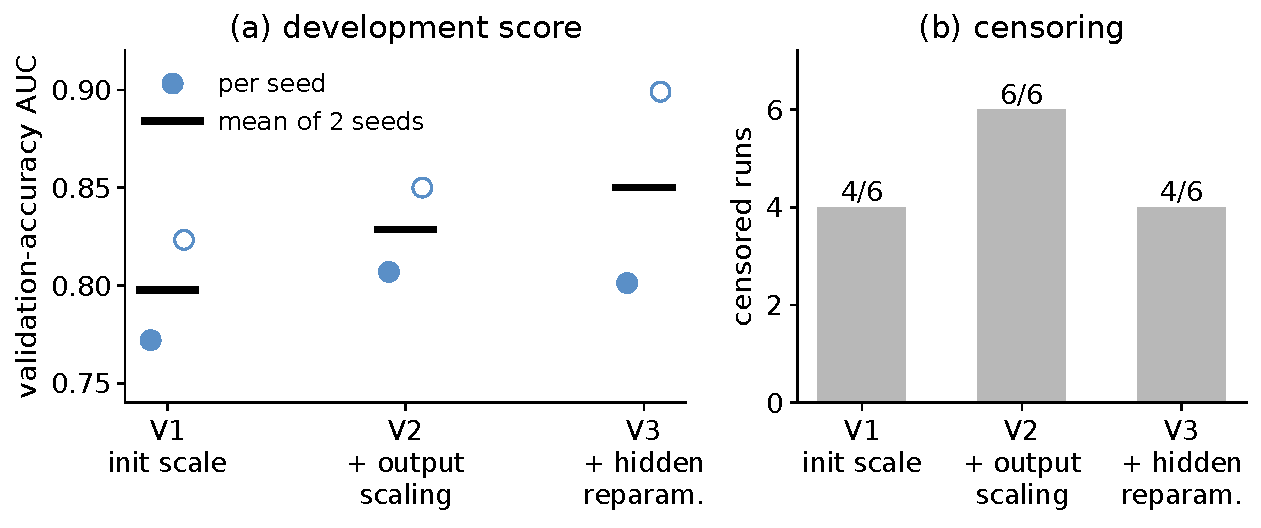
\includegraphics[width=\textwidth]{figures/search_variants_descriptive.pdf}
\caption{Development-plane comparison of three configurations (modulus $53$, training fraction $0.5$, two seeds; not the sealed evaluation). (a) Per-seed and mean held-out-accuracy AUC. (b) Number of the six runs censored at the step limit.}
\label{fig:dev}
\end{figure}

\begin{table}[h]
\centering
\caption{Development-plane summary (two seeds $\times$ three widths $=6$ runs per configuration).}
\label{tab:si-dev}
\small
\begin{tabular}{lrrrr}
\toprule
Configuration & Score & Mean final held-out acc. & Censored runs & Control max acc. \\
\midrule
V1 & $0.798$ & $0.981$ & $4/6$ & $0.023$ \\
V2 & $0.828$ & $0.944$ & $6/6$ & $0.022$ \\
V3 (evaluated) & $0.850$ & $0.921$ & $4/6$ & $0.023$ \\
\bottomrule
\end{tabular}
\end{table}

\subsection{Analyses and hypotheses not performed}
\label{sec:si-untested}
The following were considered during development and have \emph{no} results in the artifacts: a capacity-crossover account in which fitting time falls faster with width than generalization time (separate fitting and generalization steps are not retained); a critical width as a function of training fraction; a sweep of the hidden-layer exponent; a sweep of the output-scaling exponent and unembedding scale; an intervention on weight decay; and any weight-norm or circuit-level diagnostics. Nothing in the main text depends on them.

\subsection{Reproducibility}
\label{sec:si-repro}
The accompanying files are: the evaluated model's source and the two evaluators (\texttt{source\_evidence/}); the aggregate and per-seed final records (\texttt{source\_evidence/final/}); \texttt{scripts/derive\_resolution.py}, which computes every derived number in Tables~\ref{tab:resolution} and~\ref{tab:si-model} and the text from the evaluator records and writes \texttt{derived/resolution.json}; and \texttt{scripts/build\_figures.py}, which produces Figures~\ref{fig:slope} and~\ref{fig:dev} from that file. Figure~\ref{fig:overview} is a schematic with no data. Data are generated in memory from the modulus and seed, with no download. The aggregate metrics (slope, interval, reference slope, censored fraction, control, score) are those recorded by the evaluator. Re-running the evaluator requires the evaluated model's dependencies (PyTorch and NumPy); the sealed evaluation took about $3.3$ hours of wall-clock time on the recorded hardware, whose specification is not retained in the artifacts.

\subsection{LLM usage}
\label{sec:si-llm}
Large language models acted as autonomous agents in this work: they proposed the candidate directions, wrote and modified the evaluated model's code, drafted the analysis scripts, and wrote this manuscript. The task environment supplied the evaluators and the workload manifests; the models did not edit them. The interval rule that maps the evaluator's reported interval to a verdict was applied by our own script \texttt{scripts/derive\_resolution.py}. No results were produced by an LLM other than by executing the code described above, and all numbers in the paper come from the evaluator records or from the derivations in \texttt{scripts/derive\_resolution.py}.

\end{document}
